\documentclass[border=10pt]{standalone}

\usepackage{tikz}
\usepackage{tikzsymbols}
\usetikzlibrary{calc,patterns,shapes.geometric}

\def\centerarc[#1](#2)(#3:#4:#5){\draw[#1] ($(#2)+({#5*cos(#3)},{#5*sin(#3)})$) arc (#3:#4:#5);}

\begin{document}
	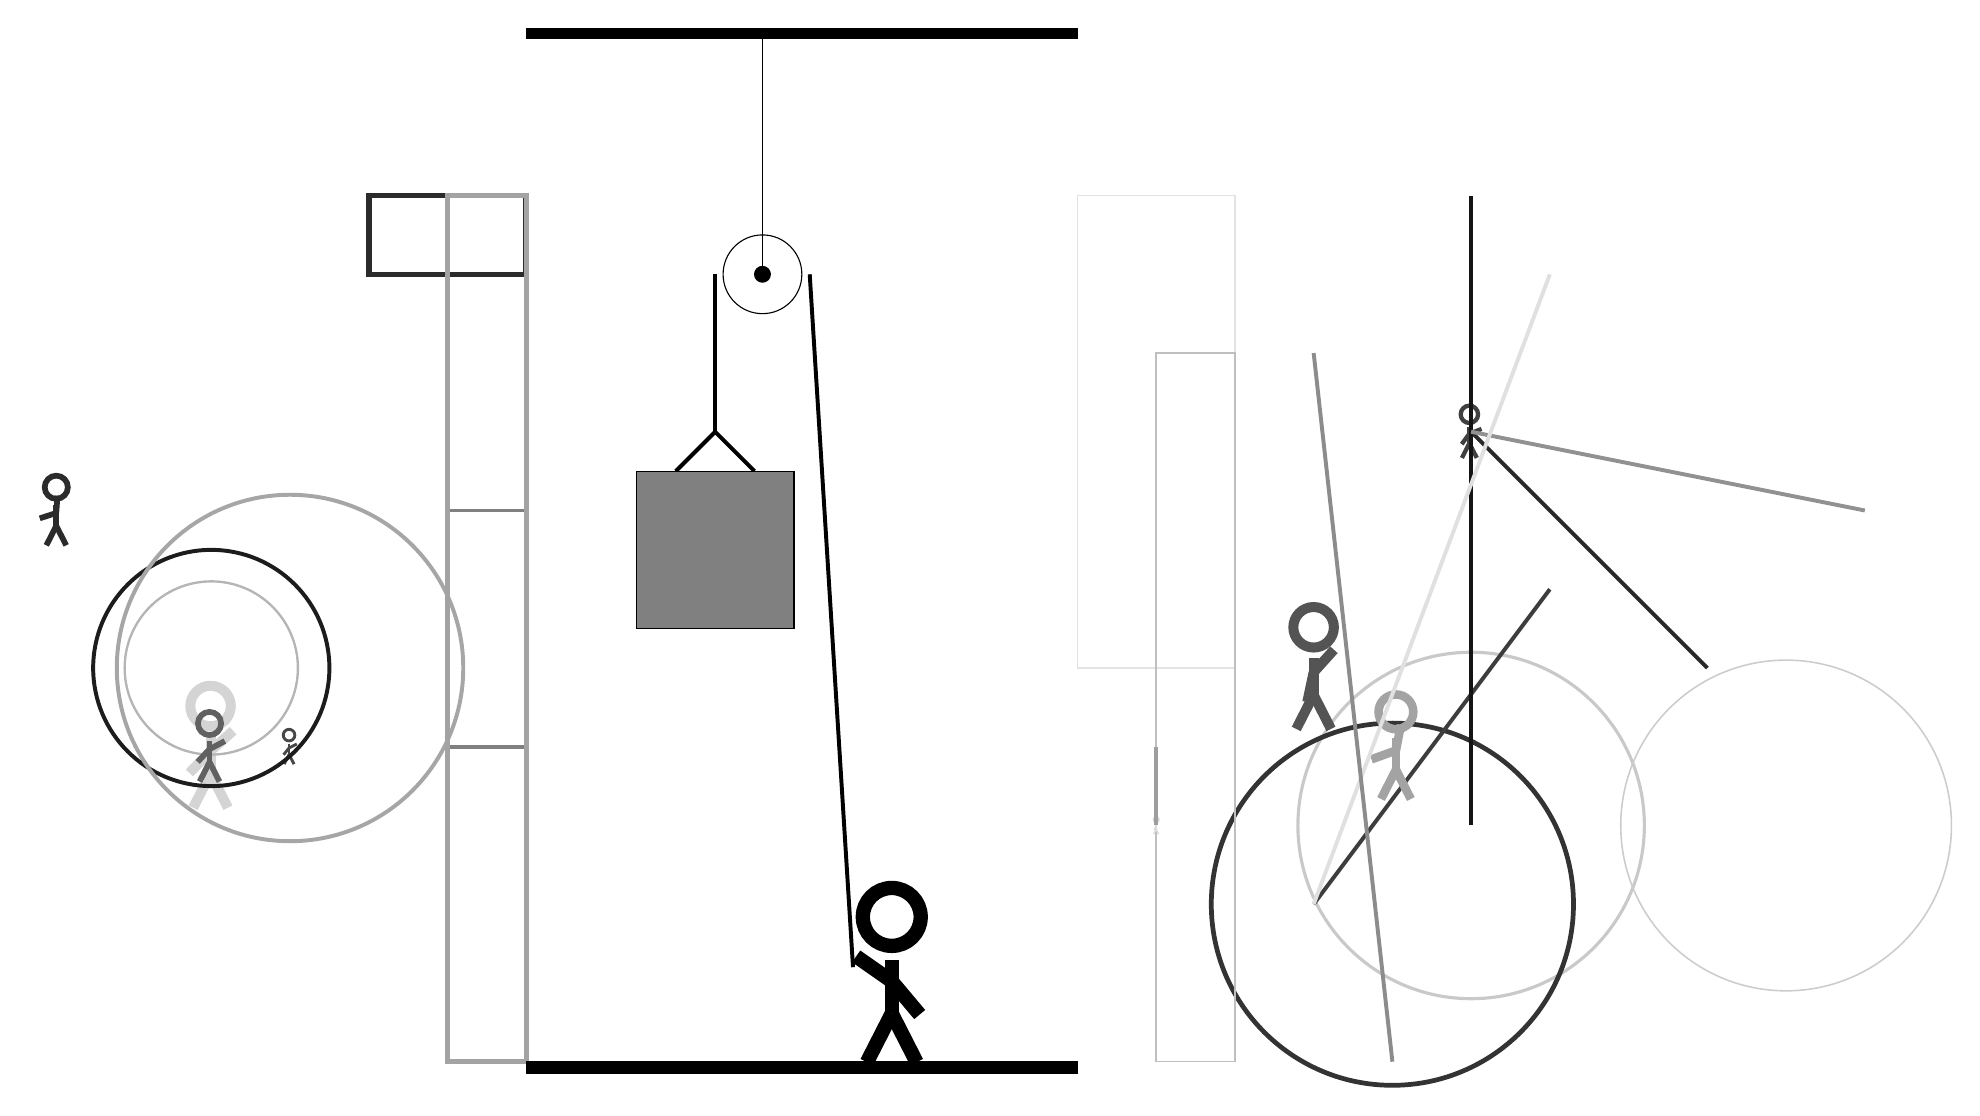
\begin{tikzpicture}
		%%%%% START %%%%%
		
		\draw[fill=black] (-2, 10) rectangle (5, 10.125);
		
		\draw (1, 7) circle (0.5);
		\draw[fill=black] (1, 7) circle (0.1);
		\draw (1, 10) -- (1, 7);
		
		\draw [line width=0.4mm, color=black!21](10, 0) circle (2.2);
		
		\draw[line width=0.2mm, color=black!11] (7, 8) rectangle (5, 2);
		\draw [line width=0.6mm, color=black!80](9, -1) circle (2.3);
		\draw[line width=0.5mm, color=black!84](10, 5) -- (13, 2);
		
		\node[line width=0.4mm, color=black!72] at (-5, 1) {\Strichmaxerl[2][51][27]};
		\draw[line width=0.2mm, color=black!25] (6, -3) rectangle (7, 6);
		
		\node[line width=0.2mm, color=black!17] at (-6, 1) {\Strichmaxerl[7][46][42]};
		
		\node[line width=0.5mm, color=black!83] at (-8, 4) {\Strichmaxerl[4][18][86]};
		\draw[line width=0.7mm, color=black!83] (-2, 7) rectangle (-4, 8);
		\draw [line width=0.5mm, color=black!89](-6, 2) circle (1.5);
		
		\draw [line width=0.3mm, color=black!29](-6, 2) circle (1.1);
		
		\node[line width=0.7mm, color=black!14] at (6, 0) {\Strichmaxerl[1][62][83]};
		\draw[line width=0.5mm, color=black!38](6, 0) -- (6, 1);
		
		\draw[line width=0.5mm, color=black!76](8, -1) -- (11, 3);
		\node[line width=0.7mm, color=black!67] at (8, 2) {\Strichmaxerl[7][78][48]};
		\node[line width=0.2mm, color=black!75] at (10, 5) {\Strichmaxerl[3][54][21]};
		\draw [line width=0.2mm, color=black!20](14, 0) circle (2.1);
		\draw[line width=0.5mm, color=black!92](10, 0) -- (10, 8);
		\node[line width=0.2mm, color=black!36] at (9, 1) {\Strichmaxerl[6][20][79]};
		\draw[line width=0.5mm, color=black!43](10, 5) -- (15, 4);
		\draw [line width=0.6mm, color=black!92](8, 0) circle (0.0);
		\node[line width=0.6mm, color=black!62] at (-6, 1) {\Strichmaxerl[4][47][28]};
		\draw[line width=0.5mm, color=black!12](8, -1) -- (11, 7);
		\draw[line width=0.5mm, color=black!50] (-2, 4) rectangle (-3, 1);
		\draw [line width=0.5mm, color=black!35](-5, 2) circle (2.2);
		
		\draw[line width=0.6mm, color=black!36] (-3, -3) rectangle (-2, 8);
		
		\draw[line width=0.5mm, color=black!45](9, -3) -- (8, 6);
		
		\draw[line width=0.5mm] (-0.1, 4.5) -- (0.4, 5.0) -- (0.9, 4.5);
		\draw[fill=black!50] (-0.6, 4.5) rectangle (1.4, 2.5);
		
		\draw[line width=0.5mm] (0.4, 7) -- (0.4, 5.0);
		\centerarc[line width=0.5mm](1, 7)(0:180:0.6);
		\draw[line width=0.5mm](1.6, 7) -- (2.15, -1.8);
		
		\node at (2.6, -1.9) {\Strichmaxerl[10][-35][-50]};
		
		\draw[fill=black] (-2, -3) rectangle (5, -3.15);
		
		%%%%% END %%%%%
	\end{tikzpicture}
\end{document}